\documentclass[10pt, a4paper]{article} 
\usepackage[
a4paper,
left=2cm,      
right=2cm,     
top=3cm,     
bottom=3cm,    
headheight=4em 
]{geometry}
\usepackage[utf8]{inputenc}
\usepackage{amsmath,amsthm,amssymb,xfrac}
\usepackage{fancyhdr}
\usepackage[hungarian]{babel}
\usepackage{graphicx}
\usepackage{float}
\usepackage{comment}
\usepackage{natbib}
\usepackage{empheq}
\usepackage{wrapfig}
\usepackage{chngcntr}
\usepackage{physics}
\usepackage{mathtools}
\counterwithin{figure}{section}
\usepackage{titlesec}
\usepackage{dsfont}
\usepackage{pdfpages}
\usepackage{t1enc}
\usepackage{tabto}
\usepackage{pgfplots}
\usepackage[colorlinks=true, 
    linkcolor=black,    % belső linkek (pl. tartalomjegyzék, képletek)
    citecolor=black,   % irodalomjegyzék hivatkozások (\cite)
    urlcolor=black   % webcímek (\url)
]{hyperref}
\graphicspath{ {./images/} }
\setlength{\marginparwidth}{0pt}
\setlength{\marginparsep}{0pt}

\pagestyle{fancy}
\fancyhf{}
\cfoot{\thepage. oldal}
\lhead{
	\textbf{Gépelemek 1. Házi feladat}
	\\Kindlik Dániel
	\\AHU27Z
}

\newcommand{\knm}{\;\mathrm{\left[kNm\right]}}
\newcommand{\kn}{\;\mathrm{\left[kN\right]}}
\newcommand{\meter}{\mathrm{\left[m\right]}}
\newcommand{\n}{\mathrm{\left[N\right]}}
\newcommand{\pknm}{\mathrm{\left[kN/m\right]}}
\newcommand{\baar}{\mathrm{\left[bar\right]}}
\newcommand{\mpa}{\mathrm{\left[MPa\right]}}
\newcommand{\mm}{\mathrm{\left[mm\right]}}
\newcommand{\mmn}{\mathrm{\left[mm^2\right]}}
\newcommand{\mmh}{\mathrm{\left[mm^3\right]}}
\newcommand{\nmm}{\mathrm{\left[Nmm\right]}}
\newcommand{\szog}{\mathrm{\left[^{\circ}\right]}}

\renewcommand*\contentsname{Tartalomjegyzék}
\begin{document}
	\begin{titlepage}
		\centering
		
\includegraphics[width=175pt]{ BMElogo.png } \\
		\vspace*{2cm}
		{\Huge \bfseries Karimás csőkötés tervezése} \\
		\vspace{0.5cm}
		{\Large Gépelemek mechatronikai mérnököknek} \\
		\vspace{0.5cm}
		{\Large 1. Házi feladat} \\
		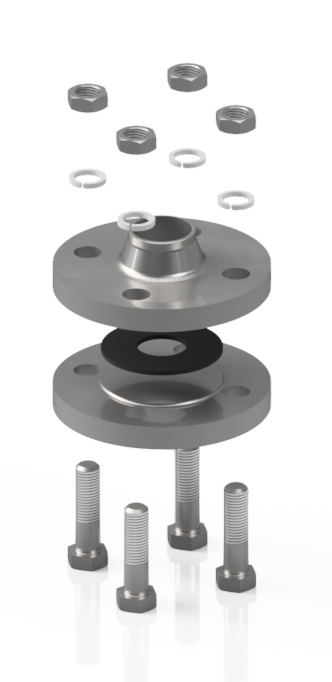
\includegraphics[width=160pt]{ osszeallitas.png } \\
		\vspace{1cm}
		{\Large \scshape Kindlik Dániel} \\
		\vspace{0.5cm}
		AHU27Z \\
		\vfill
		{\large \today} \\
	\end{titlepage}
	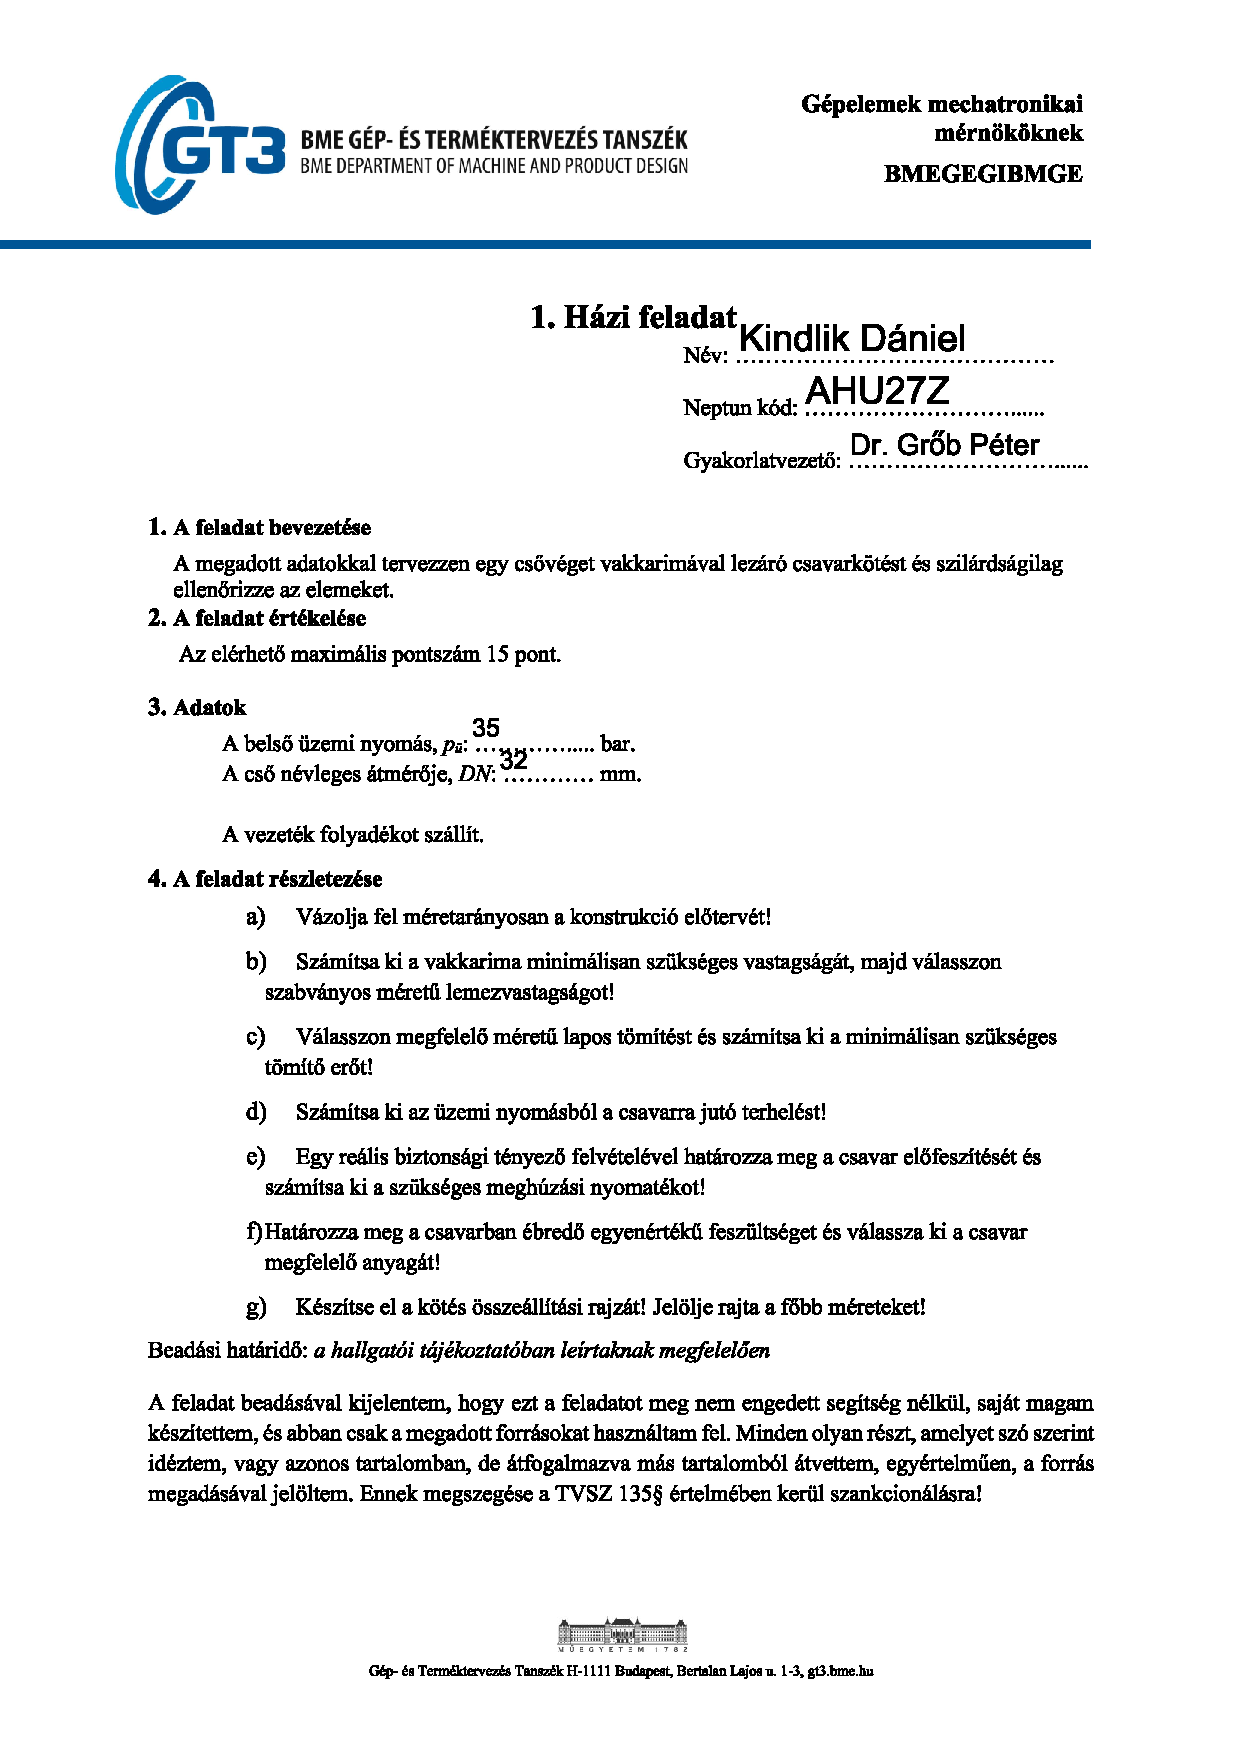
\includepdf{feladatlap.pdf}
	\thispagestyle{empty}
	\tableofcontents
	\newpage
	\setcounter{page}{3}
	\section*{Bevezetés}
	A feladat a megadott adatokkal egy csővéget vakkarimával lezáró csavarkötés tervezése és az elemek szilárdságilag
	ellenőrzése.
	\section{Előtervek}
	\subsection{Karima szabvány választása}
	A megadott adatok alapján ($p_{\ddot{u}} = 35\baar\;\;D_N = 32\mm$) ISO EN 1092-1 PN40\footnote{\url{https://globalsupplyline.com.au/wp-content/uploads/2014/10/Flange-Dim-EN1092-1-BS4504.pdf}} szabványt lett kiválasztva.
	\begin{figure}[h]
		\centering
		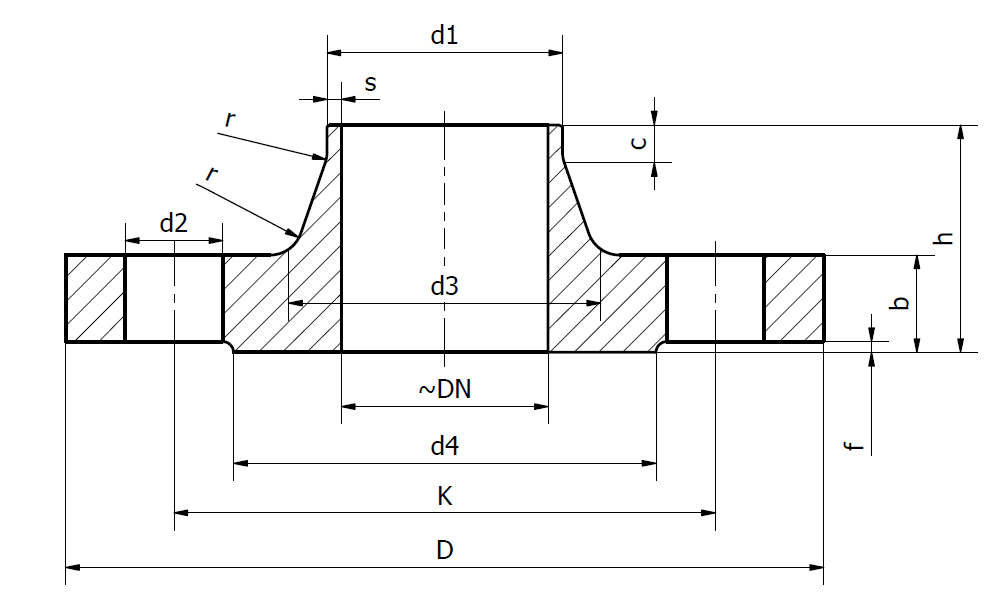
\includegraphics[width=0.6\textwidth]{ karima_eloterv.png }
		\caption{Karima előterve}
		\label{fig:karima}
	\end{figure}
	\renewcommand{\arraystretch}{1.4}
	\begin{table}[h]
		\centering
		\begin{tabular}{l|c|c}
			\textbf{Név}                              & \textbf{Jelölés} & \textbf{Érték} \\ \hline
			Karima külső átmérője                     & $D$ & 140 mm \\ 
			Karima magassága                          & $h$ & 42 mm \\ 
			Falvastagság                              & $s$ & 2.6 mm \\ 
			Kiugrás mérete                            & $f$ & 2 mm \\ 
			Kúp feletti rész magassága                & $c$                & 6 mm \\ 
			Lekerekítések nagysága                    & $r$                & 6 mm \\ 
			Cső csatlakozás külső mérete              & $d_1$             & 43.5 mm \\ 
			Csavar lyukkör átmérője                   & $d_2$             & 18 mm \\ 
			Kúp alsó átmérője                         & $d_3$             & 56 mm \\ 
			Tömítő felület külső átmérője             & $d_4$             & 78 mm \\ 
			Csavarok száma                            & $N$                & 4 db \\ 
			Csavarok mérete                           & $M$                & M16 \\ 
			Csavarok közép átmérője                   & $K$                & 100 mm \\ 
			Csavarok alapja és tömítési sík távolsága & $b$                & 18 mm \\ 
		\end{tabular}
	\end{table}
	\renewcommand{\arraystretch}{1}
	\subsection{Vakkarima szabvány választása}
	A megadott adatok alapján ($p_{\ddot{u}} = 35\baar\;\;D_N = 32\mm$) DIN EN 1092-1\footnote{\url{https://www.heco.de/en/stainless-steel/flanges/blind-flanges/din-en/more-sealing-surfaces/with-raised-face/pn-40.html}} PN40 szabványt lett kiválasztva.
	\begin{figure}[h]
		\centering
		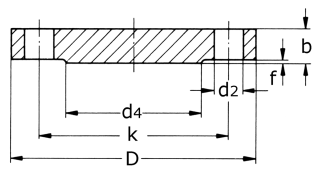
\includegraphics[width=0.4\textwidth]{ vakkarima_eloterv.png }
		\caption{Vakkarima előterve}
		\label{fig:vakkarima}
	\end{figure}
	\renewcommand{\arraystretch}{1.4}
	\begin{table}[h]
		\centering
		\begin{tabular}{l|c|c}
			\textbf{Név}                              & \textbf{Jelölés} & \textbf{Érték} \\ \hline
			Vakkarima külső átmérője                     & $D$                & 140 mm           \\
			Vakkarima magassága                          & $b$                & 18 mm			\\
			Kiugrás mérete                            & $f$                & 2 mm           \\
			Csavar lyukkör átmérője                   & $d_2$             & 18 mm           \\
			Tömítő felület külső átmérője             & $d_4$             & 78 mm           \\
			Csavarok száma                            & $N$                & 4 db           \\
			Csavarok mérete                           & $M$                & M16          \\ 
			Csavarok közép átmérője                   & $K$                & 100 mm             
		\end{tabular}
	\end{table}
	\subsection{Konstrukció előterve}
	\begin{figure}[h]
			\centering
			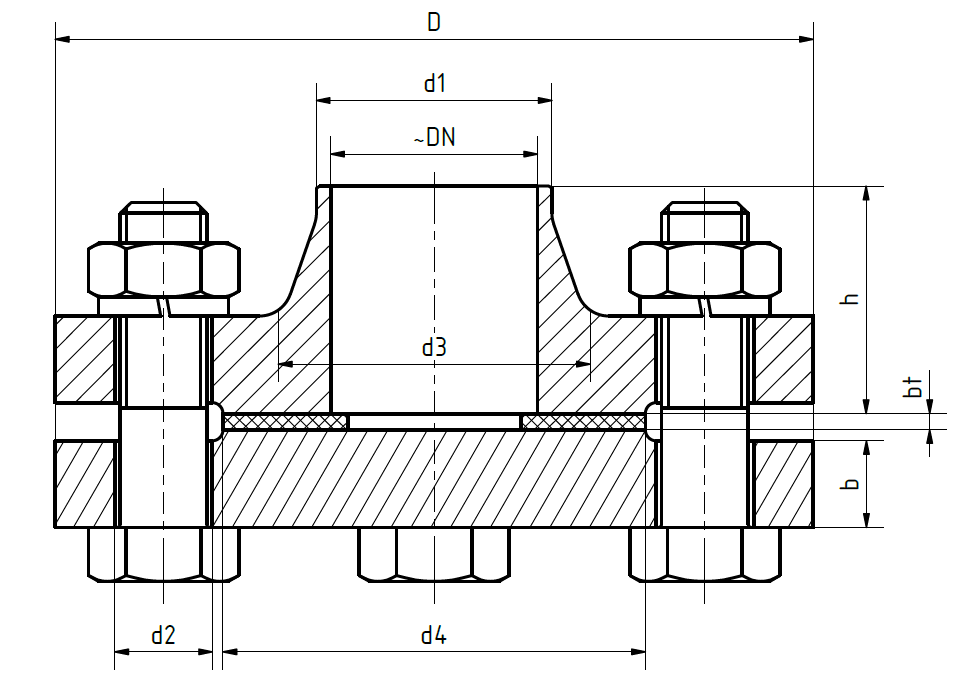
\includegraphics[width=0.5\textwidth]{ konstrukcio_eloterv.png }
			\caption{Konstrukció előterve}
			\label{fig:konstrukcio}
		\end{figure}
	\newpage
	\section{Vakkarima minimális vastagságának számítása, megfelelő lemezvastagság választása}
	A vakkarima minimális vastagságának kiszámításához használhatjuk az alábbi egyenletet:
	\begin{equation}
		b_{\text{min}} = \sqrt{\dfrac{3 \cdot p_\text{ü}}{\sigma_{\text{hajl}}} \cdot \left(1 - \dfrac{2 \cdot d_t}{3 \cdot k}\right)} \cdot \dfrac{d_t}{2} \tag{2}
	\end{equation}
	\vspace{-15pt}
	\renewcommand{\arraystretch}{1.4}
		\begin{table}[!h]
			\centering
			\begin{tabular}{l|c|c}
				\textbf{Név}                              & \textbf{Jelölés} & \textbf{M.egys.} \\ \hline
				Az üzemi nyomás                     & $p_\text{ü}$                & $\mpa$          \\
				A karima anyagára megengedhető maximális hajlító feszültség           & $\sigma_{\text{hajl}}$                & $\mpa$			\\
				A csavarok lyukkör átmérője               & $k$                & $\mm$     \\
				A tömítés középátmérője                         & $d_t$                & $\mm$           
			\end{tabular}
		\end{table}
	\renewcommand{\arraystretch}{1}\\
	$p_\text{ü}$-t át kell váltanunk MPa-ba: $p_\text{ü} = 35 \baar = 3.5 \mpa$\\\\
	$\sigma_{\text{hajl}}$ megadásához ki kell választatnunk a karima anyagát, ennek az S235 acélt választottam. $R_{eH}$ adott\footnote{Anyagok.pdf} és $n$ biztonsági tényezőnek 2-t választottam:
	\begin{equation}
		\sigma_{\text{hajl}} = \dfrac{R_{eH}}{n} = \dfrac{190}{2} = 145 \mpa \tag{2.1}
	\end{equation}
	$d_t$ kiszámolható az első feladatban megadott értékekkel:
	\begin{equation}
		d_t = \dfrac{(d_1 - 2 \cdot s) + d_4}{2} = \dfrac{(43.5 - 2 \cdot 2.6) + 78}{2} = 58.15 \mm \tag{2.2} \label{dt}
	\end{equation}
	Már mindent ismerünk $b_{min}$ kiszámolásához:
	\begin{equation}
			b_{\text{min}} = \sqrt{\dfrac{3 \cdot 3.5}{145} \cdot \left(1 - \dfrac{2 \cdot 58.15}{3 \cdot 100}\right)} \cdot \dfrac{58.15}{2} = 6.122 \mm\tag{2}
	\end{equation}
	Így láthatjuk, hogy a szabványban szereplő vastagság megfelelő.
	\newpage
	\section{Megfelelő lapos tömítés választása, minimális tömítési erő számítása}
	A minimális tömítő erő az az erő, amely a tömítőanyag összenyomásával biztosítja az üzemi nyomásnál a szivárgásmentességet. Ennek nagysága több dologtól függ. Meghatározásához az alábbi egyenletet tudjuk felhasználni:
	\begin{equation}
		F_\text{Tü} = n_t \cdot p_\text{ü} \cdot \pi \cdot d_t \cdot b_t^* \tag{3}
	\end{equation}
	\vspace{-15pt}
	\renewcommand{\arraystretch}{1.4}
			\begin{table}[!h]
				\centering
				\begin{tabular}{l|c|c}
					\textbf{Név}                              & \textbf{Jelölés} & \textbf{M.egys.} \\ \hline
					Az üzemi nyomás                     & $p_\text{ü}$                & $\mpa$          \\
					A tömítés anyagát figyelembe vevő biztonsági tényező           & $n_t$                & $\mpa$			\\
					A tömítés középátmérője               & $d_t$                & $\mm$     \\
					A tömítés hatásos szélessége                 & $b_t^*$                & $\mm$           
				\end{tabular}
			\end{table}
		\renewcommand{\arraystretch}{1}\\
	A feladat megoldásához ki kell választanunk egy tömítést, ami SBR lágytömítés\footnote{\url{https://www.tomitesgyar.hu/karima-tomites-dn-32-sbr-muszaki-gumi-tomites-32x78x30mm.html}} lett, mivel ez 40 bar nyomásig használható, így PN40-es karimákhoz jó.\\\\
	Emiatt $n_t$ értéke segédlet alapján: $n_t = 1.5$\\\\
	$b_t*$ kiszámolható az első feladatban megadott értékekkel:
	\begin{equation}
		b_t^* = 0.5 \cdot b_t = 0.5 \cdot \dfrac{78 - 32}{2} = 11.5 \mm\tag{3.1}
	\end{equation}
	Már mindent ismerünk $F_\text{Tü}$ kiszámolásához ($d_t$-t már meghatároztuk (\ref{dt})):
	\begin{equation}
		F_\text{Tü} = 1.5 \cdot 3.5 \cdot \pi \cdot 58.15 \cdot 11.5 = 11030\n\tag{3.2}
	\end{equation}
	\newpage
	\section{Csavarra jutó terhelés számítása}
	A csavarerővel biztosíthatjuk a tömítés előfeszítését és ellen tudunk tartani az használat közben fellépő erőknek. Meghatározásához az alábbi egyenletet tudjuk felhasználni:
	\begin{equation}
		F_\text{csavar szerelési} = 1.2 \cdot F_\text{csavar üzemi} = 1.2 \cdot (F_{cső} + F_p + F_\text{Tü}) \tag{4}
	\end{equation}
	\vspace{-15pt}
	\renewcommand{\arraystretch}{1.4}
			\begin{table}[!h]
				\centering
				\begin{tabular}{l|c|c}
					\textbf{Név}                              & \textbf{Jelölés} & \textbf{M.egys.} \\ \hline
					A belső nyomásból származó csőerő                     & $F_{cső}$                & $\n$          \\
					A belső nyomásból származó gyűrűfelületi erő           & $F_p$                & $\n$			\\
					Az üzemi tömítő erő              & $F_\text{Tü}$                & $\n$          
				\end{tabular}
			\end{table}
	\renewcommand{\arraystretch}{1}\\
	$F_\text{cső}$ meghatározása:
	\begin{equation}
		F_\text{cső} = \dfrac{d^2 \cdot \pi}{4} \cdot p_\text{ü} = \dfrac{(d_1 - 2 \cdot s)^2 \cdot \pi}{4} \cdot p_\text{ü} = \dfrac{(43.5 - 2 \cdot 2.6)^2 \cdot \pi}{4} \cdot 3.5 = 4032 \n\tag{4.1}
	\end{equation}
	\vspace{-15pt}
	\renewcommand{\arraystretch}{1.4}
				\begin{table}[!h]
					\centering
					\begin{tabular}{l|c|c}
						\textbf{Név}                              & \textbf{Jelölés} & \textbf{M.egys.} \\ \hline
						A cső belső átmérője                     & $d$                & $\mm$          \\
						Az üzemi nyomás erő           & $p_\text{ü}$                & $\mpa$			       
					\end{tabular}
				\end{table}
		\renewcommand{\arraystretch}{1}\\
	$F_p$ meghatározása:
	\begin{equation}
		F_p = \dfrac{(d_t^2 - d^2) \cdot \pi}{4} \cdot p_\text{ü} =  \dfrac{(58.15^2 - 38.3^2) \cdot \pi}{4} \cdot 3.5 = 5263 \n\tag{4.2}
	\end{equation}
	\vspace{-15pt}
	\renewcommand{\arraystretch}{1.4}
				\begin{table}[!h]
					\centering
					\begin{tabular}{l|c|c}
						\textbf{Név}                              & \textbf{Jelölés} & \textbf{M.egys.} \\ \hline
						A tömítés középátmérője                     & $d_t$                & $\mm$          \\
						A cső belső átmérője           & $d$                & $\mm$			\\
						Az üzemi nyomás              & $p_\text{ü}$                & $\mpa$          
					\end{tabular}
				\end{table}
	\renewcommand{\arraystretch}{1}\\
	Mostmár vissza tudunk helyettesíteni:
	\begin{equation}
		F_\text{csavar üzemi} = 4032 + 5263 + 11030 = 20325 \n\tag{4.3}
	\end{equation}
	\begin{equation}
		F_\text{csavar szerelési} = 1.2 \cdot 20325 = 24390 \n\tag{4}
	\end{equation}
	\newpage
	\section{Csavar előfeszítésének és szükséges meghúzási nyomaték számítása}
	Először a feladat megoldásához ki kell választatnunk pár hiányzó alkatrészt. A csavar a karima miatt M16-os MSZ EN ISO 4016\footnote{\url{https://www.k-mechanic.hu/kmchnc17/wp-content/uploads/2021/04/Csavarok.pdf}} szabványú hatlapfejű csavar. Ehhez egy M16-os MSZ EN ISO 4032\footnote{\url{http://glink.hu/hallgatoi_segedletek/files/2467bab9d79c9c1c6f7eb43a99cf961c.pdf} 90. oldal} szabványú csavaranyát választottam. Mindkét alkatrész menete MSZ 205 ISO\footnote{\url{http://glink.hu/hallgatoi_segedletek/files/2467bab9d79c9c1c6f7eb43a99cf961c.pdf} 99. oldal} menet.\\\\
	A meghúzási nyomaték meghatározásához az alábbi egyenletet tudjuk használni:
	\begin{equation}
		M_{megh} = M_{csavar} + M_{anya} \tag{5}
	\end{equation}
	\vspace{-20pt}
	\renewcommand{\arraystretch}{1.4}
					\begin{table}[!h]
						\centering
						\begin{tabular}{l|c|c}
							\textbf{Név}                              & \textbf{Jelölés} & \textbf{M.egys.} \\ \hline
							A csavar menetén ébredő súrlódási nyomaték                      & $M_{csavar}$                & $\nmm$          \\
							Az anya homloklapján fellépő súrlódásból eredő nyomaték           & $M_{anya}$                & $\nmm$			     
						\end{tabular}
					\end{table}
	\renewcommand{\arraystretch}{1}\\
	$M_{csavar}$ meghatározásához az alábbi képletet tudjuk felhasználni:
	\begin{equation}
		M_{csavar} = F_v \cdot \dfrac{d_2}{2} \cdot \tan(\alpha + \rho') \tag{5.1}
	\end{equation}
	\vspace{-25pt}
	\renewcommand{\arraystretch}{1.4}
						\begin{table}[!h]
							\centering
							\begin{tabular}{l|c|c}
								\textbf{Név}                              & \textbf{Jelölés} & \textbf{M.egys.} \\ \hline
								A menetszárban ébredő előfeszítő erő                     & $F_v$                & $\n$          \\
								A menet középátmérője           & $d_2$                & $\mm$			 \\
								A menetemelkedés szöge           & $\alpha$                & $\szog$			 \\
								A látszólagos súrlódási félkúpszög           & $\rho'$                & $\szog$			       
							\end{tabular}
						\end{table}
	\renewcommand{\arraystretch}{1}\\
	$F_v$-t meg tudjuk adni, ha a csavarerőt elosztjuk a csavarok számával:
	\begin{equation}
		F_v = \dfrac{F_\text{csavar szerelési}}{N} = \dfrac{24390}{4} = 6098 \n\tag{5.1.1} \label{Fv}
	\end{equation}
	Menetemelkedés szögét az alábbi módon tudjuk megadni:
	\begin{equation}
		\alpha = \atan\left(\dfrac{P}{d_2 \cdot \pi}\right) = \atan\left(\dfrac{2}{14.701 \cdot \pi}\right) = 2.48 \szog\tag{5.1.2}
	\end{equation}
	\vspace{-23pt}
		\renewcommand{\arraystretch}{1.4}
							\begin{table}[!h]
								\centering
								\begin{tabular}{l|c|c}
									\textbf{Név}                              & \textbf{Jelölés} & \textbf{M.egys.} \\ \hline
									Menetemelkedés                     & $P$                & $\mm$  \\
									A menet középátmérője                     & $d_2$                & $\mm$        	       
								\end{tabular}
							\end{table}
		\renewcommand{\arraystretch}{1}\\
	Látszólagos félkúpszög szélsőértékeit az alábbi módon tudjuk meghatározni a súrlódási tényező ismeretében\footnote{\url{https://www.k-mechanic.hu/kmchnc17/wp-content/uploads/2021/04/Csavarok_meghuzasinyomateka.pdf}}:
	\begin{equation}
		\rho'_{min} = \atan\left(\dfrac{\mu_{min}}{\cos(0.5 \cdot \beta)}\right) = \atan\left(\dfrac{0.1}{\cos(0.5 \cdot 60)}\right) = 6.587 \szog\tag{5.1.3}
	\end{equation}
	\begin{equation}
			\rho'_{max} = \atan\left(\dfrac{\mu_{max}}{\cos(0.5 \cdot \beta)}\right) = \atan\left(\dfrac{0.14}{\cos(0.5 \cdot 60)}\right) = 9.183 \szog\tag{5.1.4}
	\end{equation}
		\vspace{-20pt}
			\renewcommand{\arraystretch}{1.4}
								\begin{table}[!h]
									\centering
									\begin{tabular}{l|c|c}
										\textbf{Név}                              & \textbf{Jelölés} & \textbf{M.egys.} \\ \hline
										Menetes csatlakozásnál súrlódási tényező                     & $\mu$                & $-$        \\
										A menet profilszöge (Metrikus meneteknél 60$^\circ$)                      & $\beta$                & $\szog$       	       
									\end{tabular}
								\end{table}
			\renewcommand{\arraystretch}{1}\\
	\newpage
	Így meg tudjuk adni $M_{csavar}$ szélsőértékeit:
	\begin{equation}
			M_{csavar_{min}} = F_v \cdot \dfrac{d_2}{2} \cdot \tan(\alpha + \rho'_{min}) = 6098 \cdot \dfrac{14.701}{2} \cdot \tan(2.48 + 6.587) = 7153 \nmm\tag{5.1}
	\end{equation}
	\begin{equation}
			M_{csavar_{max}} = F_v \cdot \dfrac{d_2}{2} \cdot \tan(\alpha + \rho'_{max}) = 6098 \cdot \dfrac{14.701}{2} \cdot \tan(2.48 + 9.183) = 9252 \nmm\tag{5.1} \label{Mcsavar}
	\end{equation}
	$M_{anya}$ meghatározásához az alábbi egyenletet tudjuk felhasználni:
	\begin{equation}
		M_{anya} = F_v \cdot \dfrac{d_a}{2} \cdot \mu_a \tag{5.2}
	\end{equation}
	\vspace{-20pt}
		\renewcommand{\arraystretch}{1.4}
							\begin{table}[!h]
								\centering
								\begin{tabular}{l|c|c}
									\textbf{Név}                              & \textbf{Jelölés} & \textbf{M.egys.} \\ \hline
									A menetszárban ébredő előfeszítő erő                     & $F_v$                & $\n$          \\
									Az anya felfekvő felületének közepes átmérője          & $d_a$                & $\mm$			 \\
									Az anya alatti súrlódási tényező a felfekvő felületnél           & $\mu_a$                & $-$			 	       
								\end{tabular}
							\end{table}
		\renewcommand{\arraystretch}{1}\\
	$d_a$-t az alábbi képlettel ki tudjuk számolni:
	\begin{equation}
		d_a = \dfrac{d + s}{2} = \dfrac{16 + 24}{2} = 20 \mm\tag{5.2.1}
	\end{equation}
	\vspace{-20pt}
			\renewcommand{\arraystretch}{1.4}
								\begin{table}[!h]
									\centering
									\begin{tabular}{l|c|c}
										\textbf{Név}                              & \textbf{Jelölés} & \textbf{M.egys.} \\ \hline
										A csavaranya névleges középátmérője                     & $d$                & $\mm$          \\
										A csavaranya laptávolsága          & $s$                & $\mm$			 		 	       
									\end{tabular}
								\end{table}
			\renewcommand{\arraystretch}{1}\\
	Így meg tudjuk adni $M_{anya}$ szélsőértékeit acél-acél súrlódási tényező ismeretében\footnote{\href{https://hu.wikipedia.org/wiki/S\%C3\%BArl\%C3\%B3d\%C3\%A1s\#A\_s\%C3\%BArl\%C3\%B3d\%C3\%A1si\_k\%C3\%Bap}{https://hu.wikipedia.org/wiki/Súrlódás} - Súrlódási kúp fejezet}
	\begin{equation}
			M_{anya_{min}} = F_v \cdot \dfrac{d_a}{2} \cdot \mu_{a_{min}} = 6098 \cdot \dfrac{20}{2} \cdot 0.08 = 4878 \nmm\tag{5.2}
	\end{equation}
	\begin{equation}
			M_{anya_{max}} = F_v \cdot \dfrac{d_a}{2} \cdot \mu_{a_{max}} = 6098 \cdot \dfrac{20}{2} \cdot 0.25 = 15245\nmm\tag{5.2}
	\end{equation}
	Végül vissza tudunk helyettesíteni $M_{megh}$ képletébe, hogy meghatározzuk szélsőértékeit:
	\begin{equation}
			M_{megh_{min}} = M_{csavar_{min}} + M_{anya_{min}} = 7153 + 4878 = 12031 \nmm\tag{5}
	\end{equation}
	\begin{equation}
			M_{megh_{max}} = M_{csavar_{max}} + M_{anya_{max}} = 9252 + 15245 = 24497 \nmm\tag{5}
	\end{equation}
	\newpage
	\section{Csavar anyagának kiválasztása, benne ébredő egyenfeszültség kiválasztása}
	A csavarok igénybevételének jellege húzás és csavarás, emiatt a feszültséget az alábbi egyenlettel tudjuk meghatározni:
	\begin{equation}
		\sigma_{red} = \sqrt{\sigma^2 + 3 \cdot \tau^2} \tag{6}
	\end{equation}
		\vspace{-20pt}
			\renewcommand{\arraystretch}{1.4}
								\begin{table}[!h]
									\centering
									\begin{tabular}{l|c|c}
										\textbf{Név}                              & \textbf{Jelölés} & \textbf{M.egys.} \\ \hline
										A húzásból származó maximális feszültség                     & $\sigma$                & $\mpa$          \\
										A csavarásból származó maximális feszültség          & $\tau$                & $\mpa$			 	 	       
									\end{tabular}
								\end{table}
			\renewcommand{\arraystretch}{1}\\
	$\sigma$ az alábbi képlettel meghatározható:
	\begin{equation}
		\sigma = \dfrac{F_v}{A_e} \tag{6.1}
	\end{equation}
			\vspace{-20pt}
				\renewcommand{\arraystretch}{1.4}
									\begin{table}[!h]
										\centering
										\begin{tabular}{l|c|c}
											\textbf{Név}                              & \textbf{Jelölés} & \textbf{M.egys.} \\ \hline
											A menetszárban ébredő előfeszítő erő                      & $F_v$                & $\n$          \\
											A csavarszár egyenértékű keresztmetszete          & $A_e$                & $\mmn$			 	 	       
										\end{tabular}
									\end{table}
				\renewcommand{\arraystretch}{1}\\
	$A_e$ meghatározása:
	\begin{equation}
		A_e = \dfrac{d_e^2 \cdot \pi}{4} = \dfrac{\left(\dfrac{d_2 + d_3}{2}\right)^2 \cdot \pi}{4} = \dfrac{\left(\dfrac{14.701 + 13.546}{2}\right)^2 \cdot \pi}{4} = 157 \mmn\tag{6.1.1}
	\end{equation}
				\vspace{-20pt}
					\renewcommand{\arraystretch}{1.4}
										\begin{table}[!h]
											\centering
											\begin{tabular}{l|c|c}
												\textbf{Név}                              & \textbf{Jelölés} & \textbf{M.egys.} \\ \hline
												A menet középátmérője                      & $d_2$                & $\mm$          \\
												A menet belső átmérője          & $d_3$                & $\mm$			 	 	       
											\end{tabular}
										\end{table}
					\renewcommand{\arraystretch}{1}\\
	Így már vissza tudunk helyettesíteni $\sigma$ meghatározásához ($F_v$-t már meghatároztuk (\ref{Fv})):
	\begin{equation}
			\sigma = \dfrac{F_v}{A_e} = \dfrac{6098}{157} = 39 \mpa\tag{6.1}
	\end{equation}
	$\tau$ az alábbi képlettel meghatározható:
	\begin{equation}
		\tau = \dfrac{M_{csavar}}{K_p} \tag{6.2}
	\end{equation}
					\vspace{-20pt}
						\renewcommand{\arraystretch}{1.4}
											\begin{table}[!h]
												\centering
												\begin{tabular}{l|c|c}
													\textbf{Név}                              & \textbf{Jelölés} & \textbf{M.egys.} \\ \hline
													A csavar menetén ébredő súrlódási nyomaték                      & $M_{csavar}$                & $\nmm$          \\
													A csavarszár poláris keresztmetszeti tényezője          & $K_p$                & $\mmh$			 	 	       
												\end{tabular}
											\end{table}
						\renewcommand{\arraystretch}{1}\\
	$K_p$ meghatározása:
	\begin{equation}
			K_p = \dfrac{d_e^3 \cdot \pi}{16} = \dfrac{\left(\dfrac{d_2 + d_3}{2}\right)^3 \cdot \pi}{16} = \dfrac{\left(\dfrac{14.701 + 13.546}{2}\right)^3 \cdot \pi}{16} = 553.17 \mmh\tag{6.2.1}
	\end{equation}
	Így már vissza tudunk helyettesíteni $\tau$ meghatározásához ($M_{csavar_{max}}$-t már meghatároztuk (\ref{Mcsavar})):
	\begin{equation}
			\tau = \dfrac{M_{csavar_{max}}}{K_p} = \dfrac{9252}{553.17} = 17 \mpa\tag{6.2}
	\end{equation}
	\newpage
	Így már meg tudjuk határozni $\sigma_{red}$-t:
	\begin{equation}
		\sigma_{red} = \sqrt{39^2 + 3 \cdot 17^2} = 49 \mpa\tag{6}
	\end{equation}
	A feszültség ismeretében ki tudunk választani egy szilárdsági osztályt, aminek a 3.6-ost választottam. Ez alapján meg tudjuk határozni a folyáshatárt: $R_{eH} = 10 \cdot 3 \cdot 6 = 180 \mpa$.\\\\
	Így el tudjuk végezni az ellenőrzést, aminél $n = 2$ biztonsági tényezőt használunk:
	\begin{equation}
		\sigma_{meg} = \dfrac{R_{eH}}{n} = \dfrac{180}{2} = 90 \mpa\notag
	\end{equation}
	\begin{equation}
		\tau_{meg} = \dfrac{\sigma_{meg}}{\sqrt{3}} = \dfrac{90}{\sqrt{3}} = 52 \mpa\notag
	\end{equation}
	Láthatjuk, hogy egyik értékünk sem haladja meg a megengedettet, így a szilárdsági osztályunk megfelelő.
	\section{Konstrukció összeállítási rajza}
	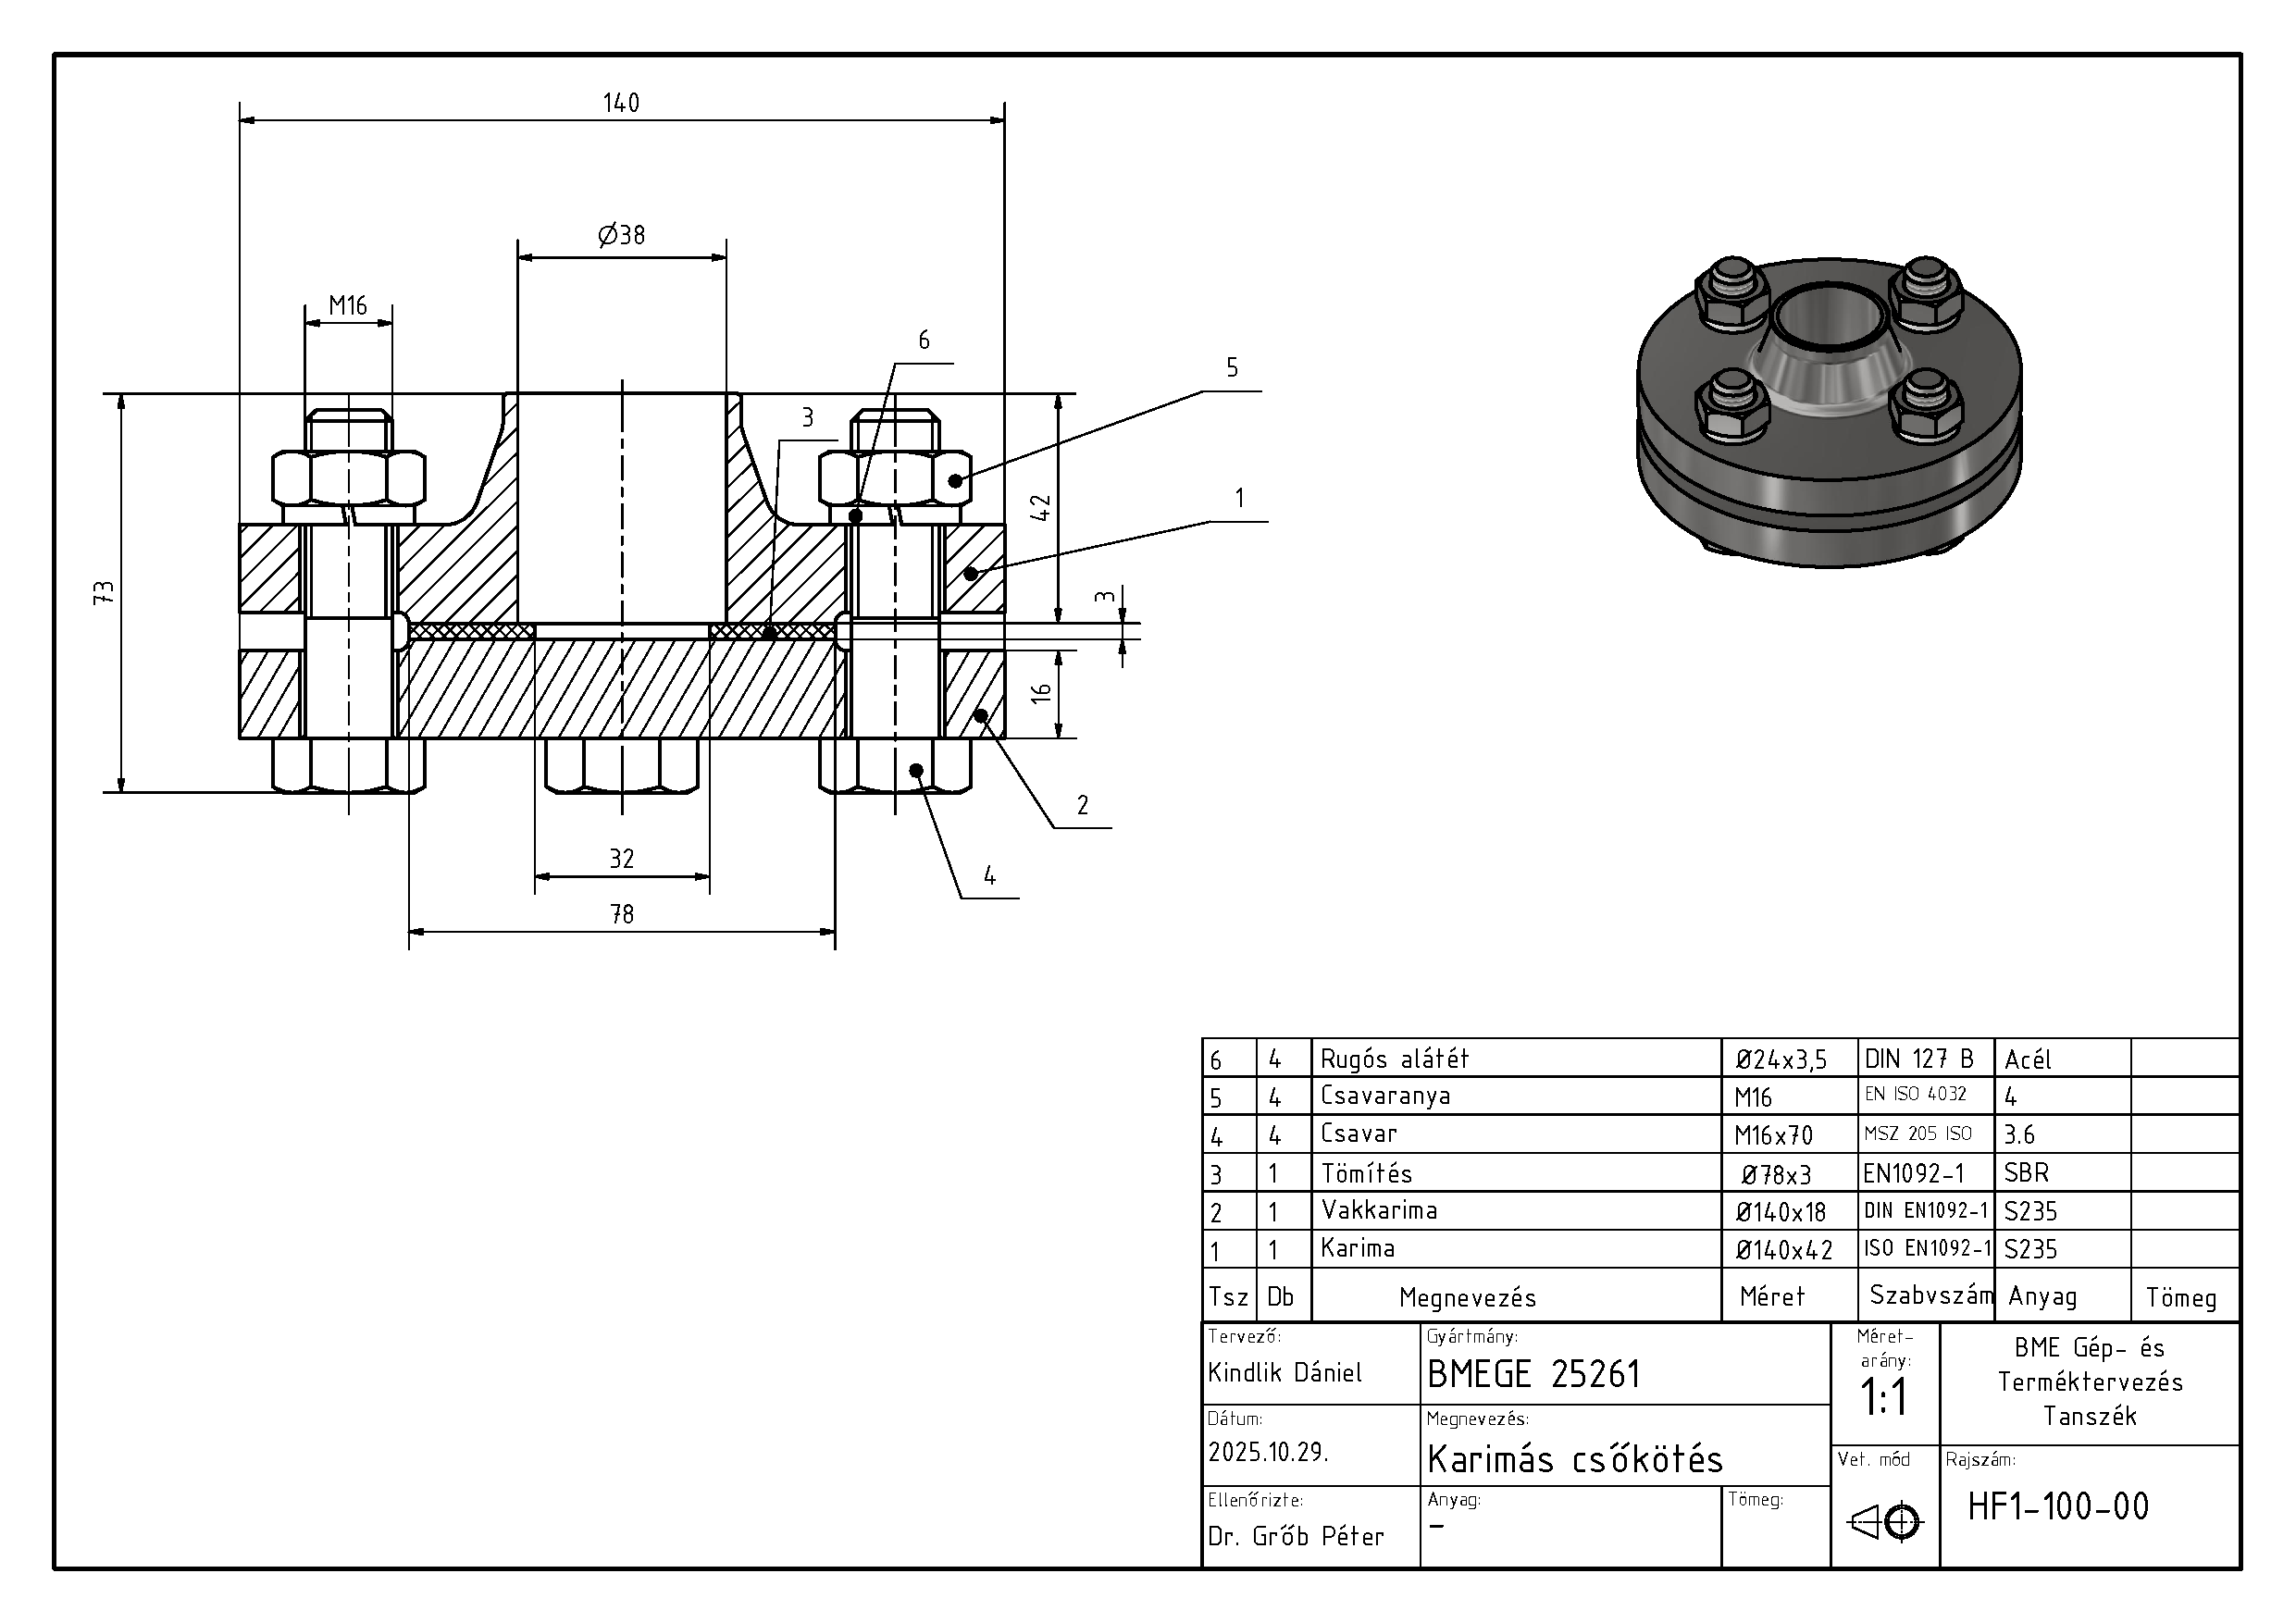
\includepdf[fitpaper]{osszeallitas.pdf}
\end{document}